\section{Métodos lineares}
A subseção \ref{subsec:cota-inferior} mostrou que a cota inferior para algoritmos baseados em comparação é $\Omega(n\log_2n)$. Isso significa que, para um algoritmo ser linear, ele não pode se basear em comparação. Além disso, os algoritmos lineares de ordenação apresentados neste trabalho só são lineares para entradas que obedecem a certas propriedades. Por exemplo, o Countingsort assume que os elementos da entrada podem ser indexados e que a diferença entre o maior e o menor elemento é limitada por uma constante suficientemente pequena para caber na memória. Já o Bucketsort requer que os elementos estejam uniformemente distribuídos em um intervalo. Por fim, o Radixsort assume que o algoritmo auxiliar é estável e linear e que cada elemento da entrada pode ser decomposto em dígitos pertencentes a um conjunto limitado e ordenável. Todos esses pré-requisitos foram levados em consideração nos testes, e todos os vetores foram gerados de modo a manter a característica linear de cada algoritmo.

\begin{figure}[H]
\Caption{\label{fig:lineares}Métodos lineares – Tempo e movimentações.}
\centering
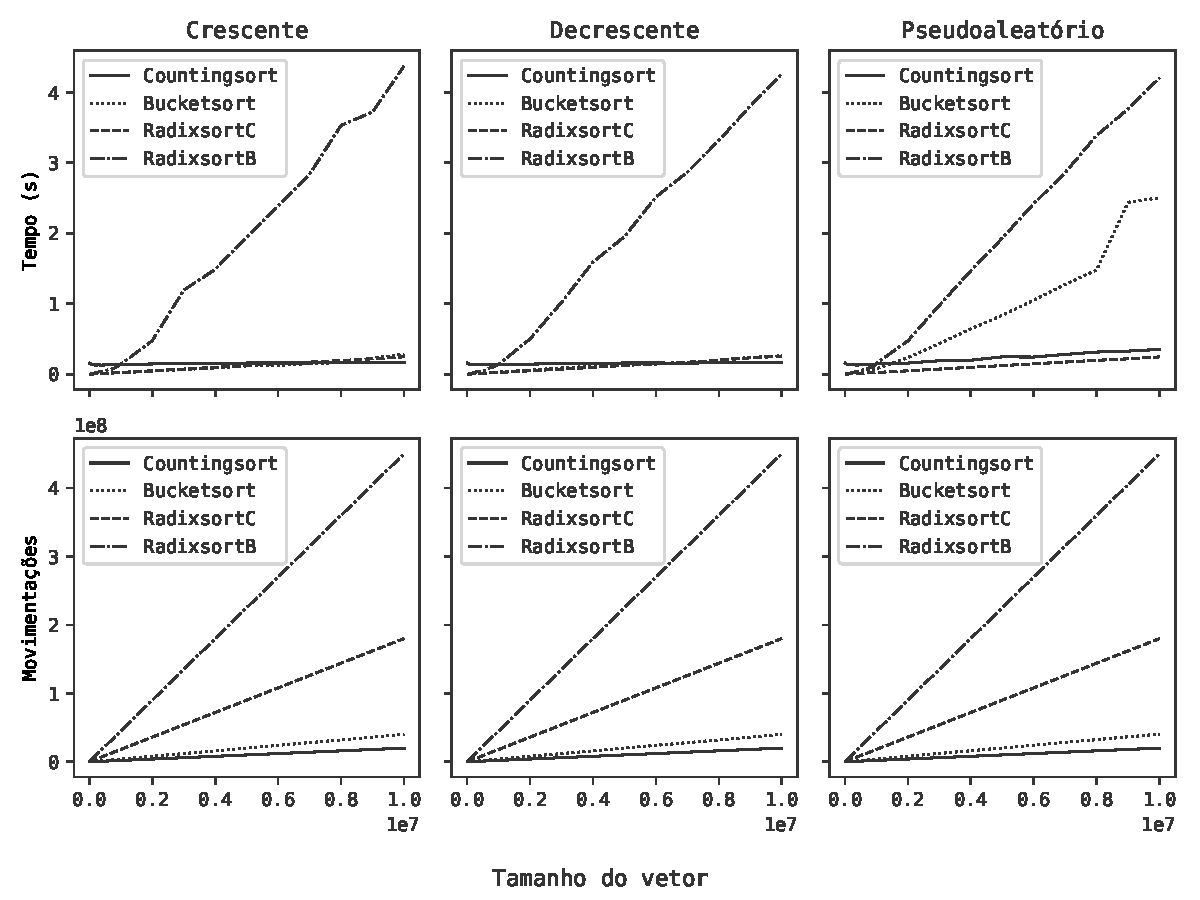
\includegraphics[scale=0.787]{figuras/pdf/lineares.pdf}
\Fonte{Elaborado pelo autor}
\end{figure}

O primeiro ponto a se observar é que cada algoritmo apresenta consistência no número de movimentações. Isso ocorre porque cada um deles, independentemente do tipo de vetor, move os dados para a memória auxiliar e, em seguida, os traz de volta para o vetor de entrada, de modo a garantir a ordenação.

No entanto, ambas as versões do Radixsort — tanto a que usa o Countingsort como sub-rotina quanto a que usa o Bucketsort — executam mais movimentações. Isso se deve ao fato de que elas têm que realizar a movimentação para a memória auxiliar nove vezes, pois essa é a quantidade máxima de dígitos que cada número da entrada pode ter.

Por fim, observamos outros dois comportamentos que o gráfico não explica. O primeiro é que o RadixsortC foi mais rápido que o Countingsort, mesmo executando mais movimentações. Isso ocorre porque o RadixsortC utiliza menos memória que o Countingsort, uma vez que o vetor que armazenaria a frequência de cada elemento da entrada no Countingsort aloca $10^8$ posições, enquanto que no RadixsortC aloca apenas $10$.

O segundo é que o Bucketsort se tornou consideravelmente mais lento para vetores gerados de forma pseudoaleatória. Isso ocorre porque, mesmo que os elementos tendam a ser igualmente prováveis na geração do vetor, não é o que ocorre exatamente na prática. Para vetores crescentes ou decrescentes, devido à forma como os elementos foram escolhidos na geração dos vetores, cada bucket recebeu entre $0$ e $2$ elementos, o que não sobrecarrega a versão do Insercao utilizada. Já para vetores gerados de forma pseudoaleatória, os buckets tiveram entre $0$ e $9$ elementos, como mostra a Figura \ref{fig:frequencia-buckets}. Esse desequilíbrio fez com que o Insercao precisasse executar mais operações na lista ligada utilizada, o que tornou o algoritmo mais lento nesses casos.

\begin{figure}[H]
\Caption{\label{fig:frequencia-buckets}Bucketsort – Frequência de tamanho de bucket ($10^7$ elementos)}
\centering
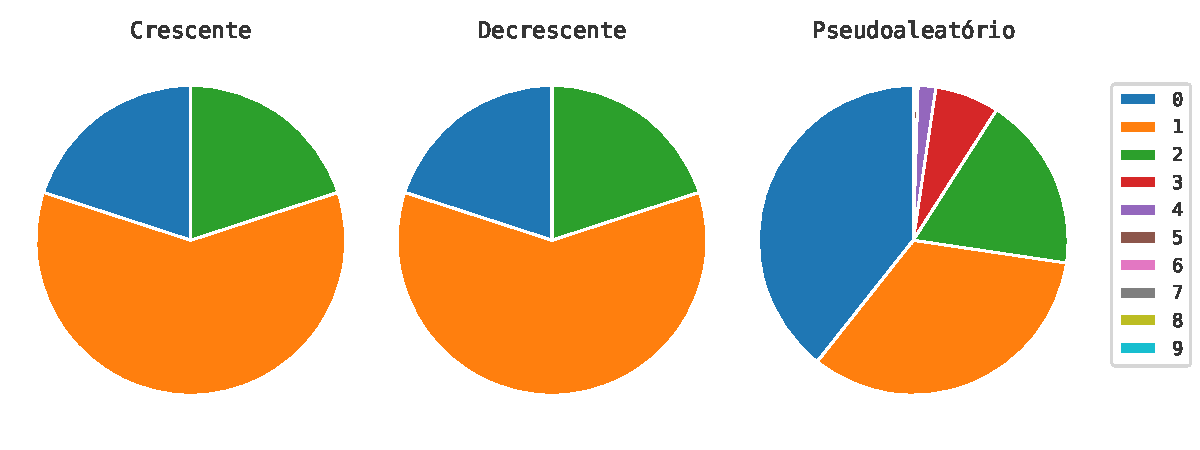
\includegraphics[scale=0.787]{figuras/pdf/frequencia_buckets.pdf}
\Fonte{Elaborado pelo autor}
\end{figure}
